\subsubsection{Sequential Models} \label{sec:theory-approach-methodology-sequential-models}

\begin{figure}[t]
	\centering
	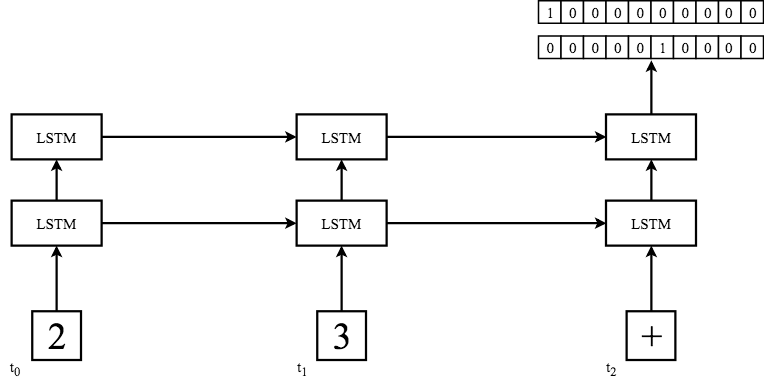
\includegraphics[max width=\textwidth]{sequential-model-arithmetic}
	\caption{A deep LSTM network that accepts a sequence of two operands and learns to perform addition on them.}
	\label{fig:sequential-model-arithmetic}
\end{figure}

When humans perform arithmetic operations, like addition, they tend to read an operand, followed by an operator, followed by another operand and then they perform the operation and produce an output. This approach to arithmetic is sequential in nature and depends on our ability to retain a representation of the operands in our minds as we read them, before we perform the operation. Given that recurrent neural networks are better suited to modeling these kinds of sequential processes, as discussed in Section \ref{sec:background-sequence-modeling}, we therefore opted to using recurrent neural networks for our experiments.

Figure \ref{fig:sequential-model-arithmetic} shows how the arithmetic expression 2 + 3 = 5 can be modeled using recurrent neural networks. On each time step the model accepts a 28x28 image of a handwritten digit from the MNIST dataset. On the last time step the model receives the operator, again in the form of a 28x28 image, and produces an output which is the result of performing the operation on the two operands. The result is represented using a pair of one-hot vectors, one vector represents the least significant digit of the result and the other represents the most significant digit of the result. Notice that we provide the operator on the final time step as opposed to the middle time step. This is because we use reverse Polish notation (RPN) when presenting the operations to the neural networks.

\paragraph{Reverse Polish Notation}

The reverse Polish notation (RPN) is a notation used to depict arithmetic expressions without the need for parentheses to indicate precedence. Unlike traditional mathematical notation where the operands of a binary operator are placed on the left and right of the operator, in RPN both operands precede the operator. The expression
\begin{gather*}
	(7 + 5) - 2
\end{gather*}
would be expressed as
\begin{gather*}
	7\ 5\ +\ 2\ -
\end{gather*}
As long as the operations have a non-variable number of operands, any arbitrarily long sequence of operations can be represented in RPN\cite{wiki:reverse-polish-notation}.

Early stack based computer models based on the work of Dijkstra and Bauer utilized RPN to reduce memory access while evaluating mathematical expressions\cite{wiki:reverse-polish-notation}. Hence, we believe that using RPN to train neural networks to perform arithmetic operations would reduce the complexity of the problem, making it easier to investigate the core hypothesis of this thesis and focus on contrasting the models' accuracy due to the presence of symbols or lack thereof instead of worrying about other factors.